% Full seminar: preserve each supplied PDF's layout and use continuous numbering.
% Edit the three source decks in their own folders, rebuild them, then rebuild here.
\documentclass{article}
\usepackage[utf8]{inputenc}
\usepackage[T5]{fontenc}
\usepackage[vietnamese]{babel}
\usepackage{lmodern}
\usepackage[paperwidth=160mm,paperheight=90mm,margin=0pt]{geometry}
\usepackage{pdfpages}
\usepackage{tikz}
\usepackage[unicode,bookmarksopen=true,bookmarksnumbered=false]{hyperref}
\hypersetup{
 pdftitle={Quản lý và Lập lịch GPU cho AI Workloads trên GKE},
 pdfauthor={Trần Nguyễn Việt Hưng; Nguyễn Hoàng Gia Huy; Nguyễn Đình Minh},
 pdfsubject={Kueue, Gang Scheduling, Topology-Aware Scheduling, GPU Sharing},
 pdfdisplaydoctitle=true,
 pdfpagemode=UseOutlines,
 pdfstartview=Fit,
 pdfpagelayout=SinglePage
}
\pagestyle{empty}
\definecolor{SeminarBlue}{RGB}{30,78,121}
\definecolor{SeminarMuted}{RGB}{87,105,122}
\newcommand{\SeminarPageTotal}{34}
% Replace only the original local page number, preserving the other footer content.
\newcommand{\LightPageNumber}{%
 \thispagestyle{empty}%
 \begin{tikzpicture}[remember picture,overlay]
  \ifnum\value{page}>27\relax
   % The supplied Part 3 uses a wider date footer; align it with Part 1.
   \fill[white] ([xshift=-4.2cm,yshift=.09cm]current page.south east)
    rectangle ([xshift=-.60cm,yshift=.60cm]current page.south east);
   \node[anchor=base east,inner sep=0pt,text=SeminarMuted,
    font=\sffamily\fontsize{7}{8}\selectfont]
    at ([xshift=-1.78cm,yshift=.21cm]current page.south east)
    {November 27\textsuperscript{th} 2026};
  \else\ifnum\value{page}>2\relax\ifnum\value{page}=27\relax\else\ifnum\value{page}=11\relax\else
   \fill[white] ([xshift=-1.35cm,yshift=.09cm]current page.south east)
    rectangle ([xshift=-.60cm,yshift=.54cm]current page.south east);
  \fi\fi\fi\fi
  \node[anchor=base east,inner sep=0pt,text=SeminarMuted,
   font=\sffamily\fontsize{7}{8}\selectfont]
   at ([xshift=-.65cm,yshift=.21cm]current page.south east)
   {\thepage\,/\,\SeminarPageTotal};
 \end{tikzpicture}}
\newcommand{\BluePageNumber}{%
 \thispagestyle{empty}%
 \begin{tikzpicture}[remember picture,overlay]
  \fill[SeminarBlue] ([xshift=-1.35cm]current page.south east)
   rectangle ([yshift=.28cm]current page.south east);
  \node[anchor=base east,inner sep=0pt,text=white,
   font=\sffamily\bfseries\fontsize{6}{7}\selectfont]
   at ([xshift=-.19cm,yshift=.09cm]current page.south east)
   {\thepage\,/\,\SeminarPageTotal};
 \end{tikzpicture}}
\begin{document}

\includepdf[pages=-,pagecommand={\LightPageNumber},
 addtotoc={1,section,1,{Phần 1: Kubernetes, Gang Scheduling và Kueue},part-one}]
 {Cloud_Part1/cloud-part1.pdf}
% Part 2 divider: reuse the background, left stripe and title typography of Part 1.
\clearpage
\thispagestyle{empty}
\null
\pdfbookmark[0]{Phần 2: Distributed Training và Topology-Aware Scheduling}{part-two}
\begin{tikzpicture}[remember picture,overlay]
 \node[opacity=.12,inner sep=0] at (current page.center)
  {
\includegraphics[width=\paperwidth,height=\paperheight]{Cloud_Part1/assets/Background.pdf}};
 \fill[white] (current page.north west)
  rectangle ([yshift=-.92cm]current page.north east);
 \fill[SeminarBlue] (current page.north west)
  rectangle ([xshift=.38cm]current page.south west);
 \node[align=left,anchor=west,text=SeminarBlue,
  font=\sffamily\fontsize{30}{37}\selectfont\bfseries,text width=13.3cm]
  at ([xshift=1.3cm]current page.west)
  {Distributed Training\\\& Topology-Aware\\Scheduling};
\end{tikzpicture}
\LightPageNumber
\clearpage
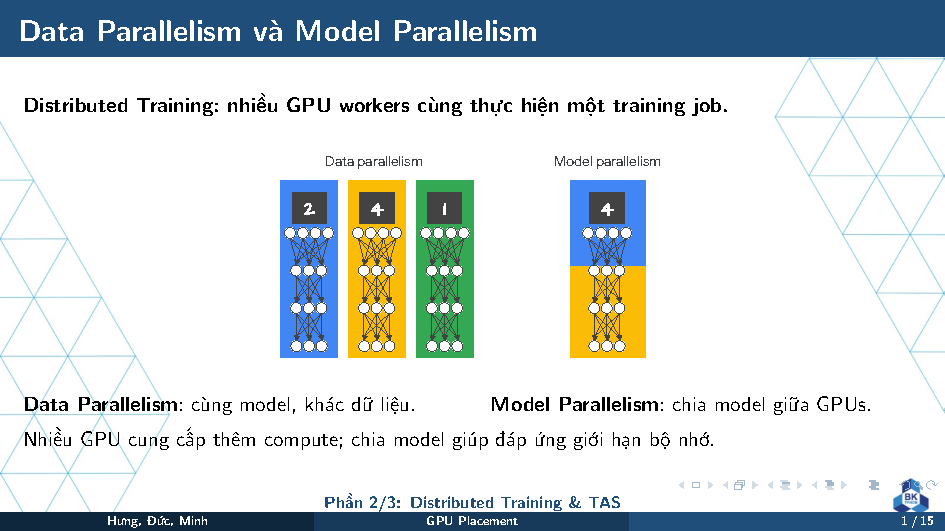
\includepdf[pages=-,pagecommand={\BluePageNumber}]
 {Cloud_Part_2/main.pdf}

\includepdf[pages=-,pagecommand={\LightPageNumber},
 addtotoc={1,section,1,{Phần 3: GPU Sharing và Resource Optimization},part-three}]
 {Cloud_Part3/cloud-part3.pdf}
\end{document}
